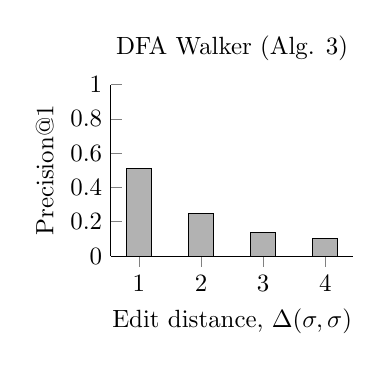
\begin{tikzpicture}[scale=0.9]
  \begin{axis}[
  ybar,
  xlabel={Edit distance, $\Delta(\err\sigma, \sigma)$},
  ylabel={Precision@1},
  title={DFA Walker (Alg. 3)},
  axis x line*=bottom,
  axis y line*=left,
  ymin=0,
  ymax=1,
  xtick=data,
  xticklabels={1, 2, 3, 4},
  width=5cm,
  height=4cm,
  enlarge x limits=0.15,
  legend style={at={(0.5,-0.15)},
  anchor=north,legend columns=-1},
  ]
  \addplot[fill=black!30] table[x=Lev, y=P@1] {
    Lev P@1
    1 0.51
    2 0.25
    3 0.14
    4 0.10
  };
  \end{axis}
\end{tikzpicture}

%Δ(1)= Top-1/total: 147 / 148 = 0.99
%Δ(2)= Top-1/total: 166 / 168 = 0.99
%Δ(3)= Top-1/total: 96 / 150 = 0.64
%Δ(4)= Top-1/total: 26 / 152 = 0.17